\chapter{Bevezetés}

Ebben a fejezetben betekintést nyújtok az olvasó számára a feladatról, mint problémáról, hogy az miért is indokolt és milyen iparágakat érinthet, mi a pontos célja a feladatnak és mik a főbb kritériumok. Tisztázni szeretném a képet az olvasóban, hogy mik is a projekt előzményei amely alapján kialakult a feladatspecifikáció és mi is az a motiváció ami pontosan ezt a projektet eredményezte.

\section{Előzmények}

A témám címe felhő alapú drónvezérlés, aminek tükrében többféle ágazatból is belecsöppenhettem ennek a projektnek a feladatköreibe. Ugyanis a felhőtechnológiák, a robotvezérlés és az irányítástechnika spektrumot is lefedi a feladat, azonban én a felhőtechnológiák felől közelítem meg. Villamosmérnök BSC 5. félévében témalabor keretei között csatlakoztam a Távközlési és Médiainformatika Tanszék (TMIT) Felhő alapú hálózatok szakmai műhelyéhez, ahol azóta is minden félévben végzek projektfeladatot. Ehhez a motivációm egyszerű volt, mivel már az alapképzés eleje óta érdekelnek azon architektúrák, ahol erőforrás menedzselés és központi irányítás alatt, például master-slave módon működnek. A felhőalkalmazások ipara is egy ilyen terület, ahol bizonyos szolgáltatásokat minél szélesebb körben szeretnénk értékesíteni igény szerint, azonban valamilyen központi vezérlés működteti automatikusan az erőforráskiosztást, hozzáférést. A műhelyben végzett feladataim között felmerült a Kubernetes elosztott konténerkezelő rendszer, a Kubless serverless architektúra, felhő alapú beszédfelismerő rendszerek és az OpenStack virtuális gép menedzselő rendszer, amihez egy archiválási megoldást fejlesztettem szakdolgozatként. A felhő alapú drónirányítás téma a diplomatervem kezdetén került szóba, előtte nem foglalkoztam mélyebben robotirányítással és vezérléssel, így remélhetőleg ezekből a területekből is nagy tapasztalatot fogok szerezni a feladat befejeztén.

\section{A feladat célja}

A feladat sokféleképpen általánosítható, hiszen egy felhőrendszerből igen sokféle ipari folyamatot lehet irányítani, csupán a megvalósítást kell kivitelezni. Egy drón irányítása sem különbözik, lehetne a cél robotkar vezérlése, gyártósor ütemezése, automatikus kötöttpályás közlekedési eszköz irányítása vagy akár önvezető autók feletti vezérlés.
 Azonban a témámban nem egy drón irányítását, hanem több, akár tíz-húsz, de akár százat is elérheti az a teszteset amire szeretnék megoldást adni. Egy ilyen rendszert irányító felhő architektrúban rugalmasabb és erőforrás takarékosabb üzemeltetést lehet elérni. A számításkapacitás optimalizáció nem minden amit ebben a helyzetben az ipar megkíván, hanem azokat a kommunikációs kapcsolatokat, amelyek szigorú minőségi elvárásoknak (Quality -of Service – QoS) kell megfelelniük, ezért bonyolultabb kezelni. A feladat feltérképezni a modern felhőrendszereket, amelyekkel meg lehet valósítani efféle iparban is használható vezérlési technikát QoS feltételek mellett. Tehát a projektnek három kritikus tervezési mérföldköve van. Ezeknek kapcsolata látszik a \ref{fig:merfold}. ábrán.
\begin{figure}
	\centering
	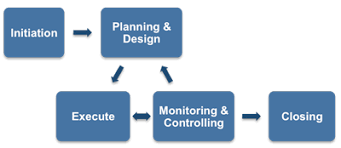
\includegraphics[width=10cm]{figures/plan_excecute_monitor.png}
	\caption{Kritikus mérföldkövek folyamata \cite{ProjecPlan}}
	\label{fig:merfold}
\end{figure}
\begin{enumerate}
	\item Kiválasztani a megfelelő felhőrendszert, amiben megvalósítható $R\in [1, 100]$ drón, vagy általánosan, valamilyen vezérelhető eszköz (robot) irányítása.
	\item Áttekinteni drónvezérlést támogató szoftver megoldásokat, kiválasztani egy olyan környezetet, mellyel távvezérlési funkciók megvalósíthatók. Megtervezni ebben a felhőrendszerben több drón irányítását és jelfeldolgozását, automatikusan és biztosítva, hogy hiba esetén visszaálljon a működő állapot.
	\item A meglévő rendszer analizálása, optimalizálása és egy QoS feltétel felállítása.
\end{enumerate}


Tehát a dolgozat célja nem csak a megvalósítás, hanem $R$ számú tízes-százas nagyságrendű robotok irányításának a QoS feltételét és validációját is megadja. Ezt a feltételt valamilyen $f_{QoS}(R,C)\in N^2$ függvény fogja megadni, melynek paraméterei $R$ a robotok száma és $C$ a számítási erőforrás. Ha számításról beszélünk, akkor a felhőszolgáltatások iparában kiválasztunk egy valamilyen optimális $c=$RAM[GB]/VCPU arányt mely az alkalmazásunkhoz megfelelő és annak $n\in N^+$, $C=c\cdot n$ egész számú többszöröse lesz a számítási kapacitás amire méretezünk. Vagyis valamilyen 2 dimenziós tervezési teret adunk meg a kívánt szolgáltatási minőség eléréséhez. Az ilyen jellegű feladatokban a szolgáltatás minősége általában a válaszidőt szokta jelenteni $n \cdot 10$-es nagyságrendben. Természetesen ez nem egy túl pontos modell, de egy mérnöki kapacitástervezés számára kellő kiindulási alapot adhat méretezni a felhőrendszert, esetleg skálázhatósági lehetőségeket is figyelembe véve.
Ezen kívül mivel nagyszámú eszközről beszélünk nem tekinthetünk el a közegátviteli technológiáról. Azt sejthetjük, hogy a mai elterjedt távközlő rendszerek nem alkalmasak akár száz fölötti felhasználóval, mondjuk robottal folyamatos kommunikációt tartani megfelelő QoS-el. Ezért megnézzük, hogy a mai modern felhőrendszerekkel és az 5G között milyen kapcsolatot lehet alakítani és mik a feltételek egy ilyen rendszerben való üzemeltetéshez.

\section{Feladat indokoltsága}
\begin{figure}
	\centering
	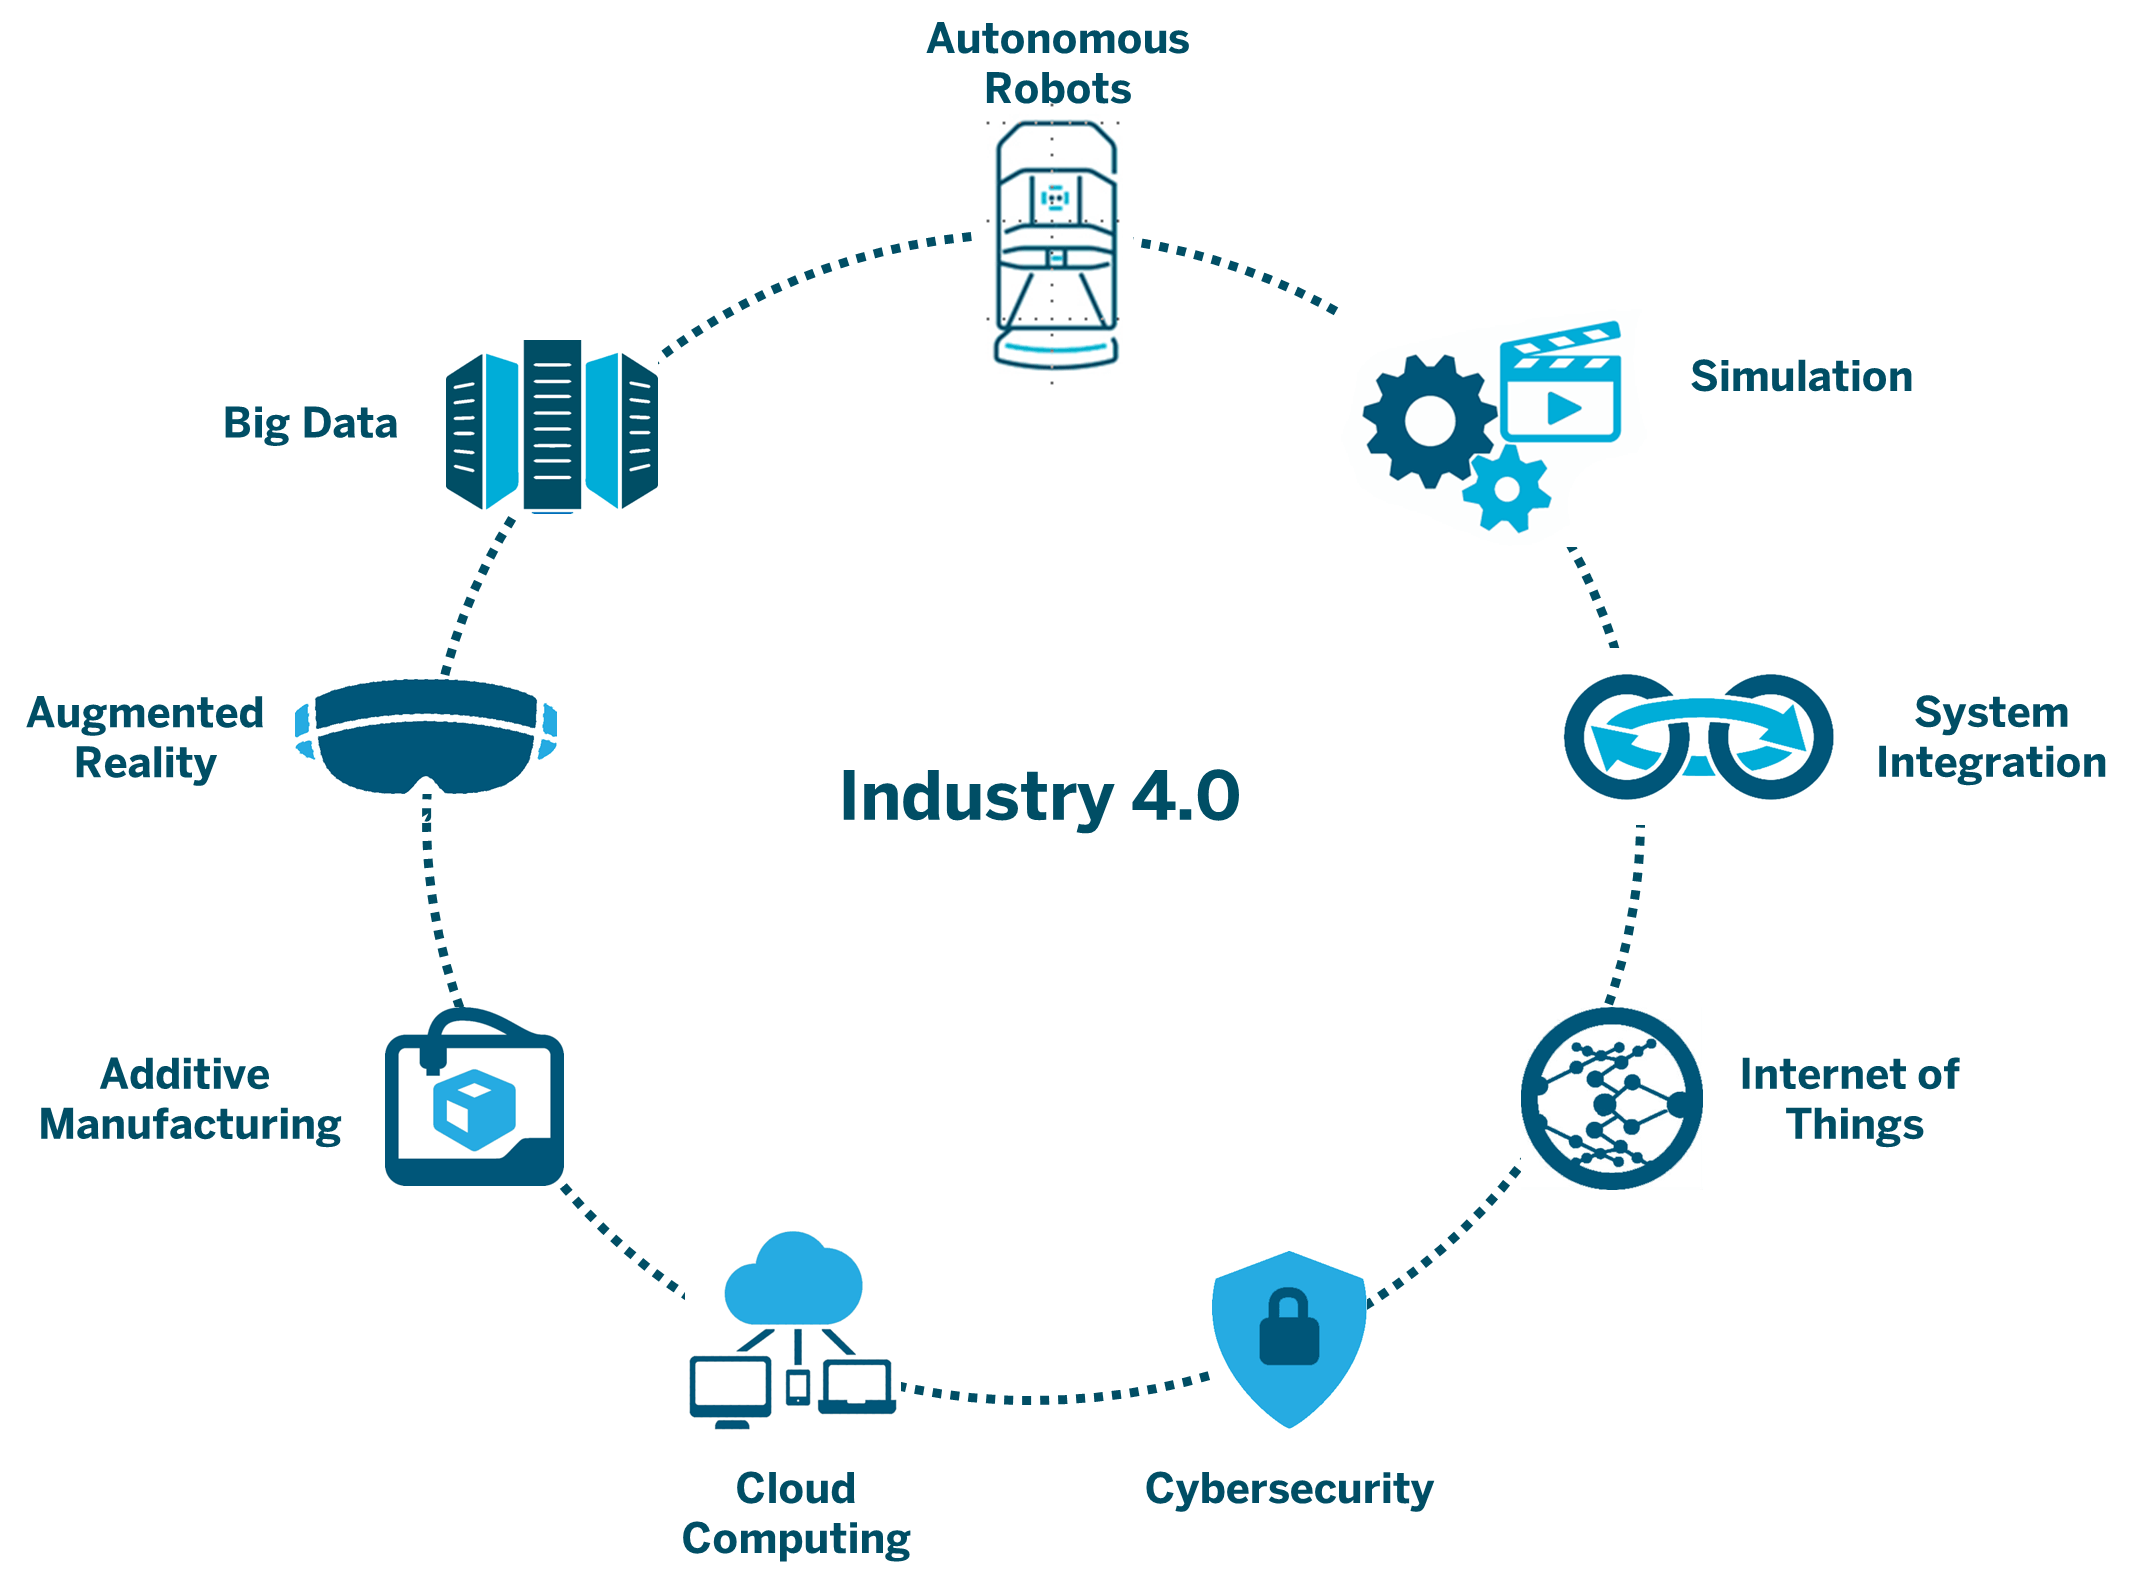
\includegraphics[width=\linewidth]{figures/industry40.png}
	\caption{Ipar 4.0 komponensei \cite{industry40}}
	\label{fig:industry40}
\end{figure}
\subsection{Gyártóipar}
A nagyszámú eszközök irányítása számtalan szektorban elterjedt és alkalmazható. Akár beszélve a gyártó szektorról, ahol nagyon sok folyamatot robotok látnak el és legyen az bármilyen robot, az valószínűleg irányítható felhőből. Persze sokszor a gyártók egy drágább, de kapacitásban túlbiztosított lokális rendszerről irányítják a gyártórobotjaikat, mivel a felhős megoldások még annyira nem elterjedtek ebben a célfelhasználásban. Azonban egy ilyen megoldással rengeteg erőforrás megtakarítható.
A \ref{fig:industry40}. ábrán láthatóak az Ipar 4.0 főbb komponensei és könnyen meggyőződhetünk róla, hogy egy mai innovatív ipari környezetben inkább a felhő alapú megoldásokat választják a skálázhatóság és a biztonságuk miatt. Ebben az esetben felhőről általában számítási kapacitásról beszélünk, azonban később kitérünk a szolgáltatások kategóriáira.

\subsection{Szállítás}
Nem csak a gyártóiparban lehet elképzelni sok robot irányítását, hanem például szállítás és utazás terén is. A Műegyetemhez legközelebbi metróvonal már évek óta önvezérlőként működik, ugyan egyelőre a hossza befejezetlensége miatt csak tíz körüli metrószerelvény működik egyszerre, azonban ez is egy olyan példája a robotirányításnak, amit minden nap észlelhetünk. Az Amazon házhozszállító cég, amelynek egyébként az AWS (Amazon Web Services) leányvállalata a világ egyik legnagyobb felhőszolgáltatója, már tesztel drónokat, amelyek betöltik a csomagházhozszállítás szerepet. A levegőben való csomagszállítás egyik problémája a \ref{fig:drone-delivery}. ábrán látható.
\begin{figure}
	\centering
	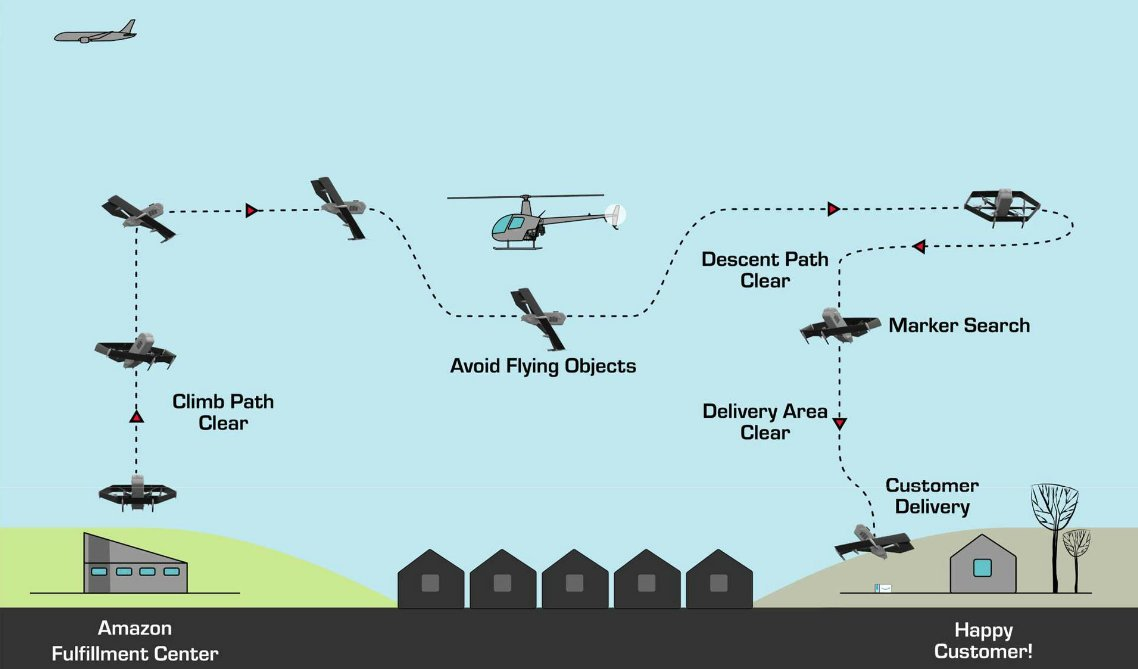
\includegraphics[width=\linewidth]{figures/aws-drone-delivery.jpg}
	\caption{Amazon házhozszállítás problémája drónnal \cite{drone-delivery}}
	\label{fig:drone-delivery}
\end{figure}
\subsection{Mezőgazdaság}
Az agrárvilágban is el lehet képzelni sok robotot kezdve a vetéstől az aratásig, azonban a drónoknak kifejezett szerepe akad a jövőben ebben az iparágban. Használnak ma már automatizált drónokat permetezésre, időszakos állomány megfigyelésre vagy akár kombájn útjának a felderítésére is. Ahogyan a gyártósoroknál, itt is optimalizálhatunk több robot irányítás esetén felhőrendszerrel. A dolgozatban arra keresünk megoldást, hogy ezt milyen eszközrendszerrel érdemes tervezni.
\subsection{Szórakoztatóipar}
Idáig kiderült, hogy rengeteg iparágban alkalmazhatóak a tömegesen irányított robotok, amiket kreativitással könnyű bővíteni. Azonban a szórakoztatóiparban is megjelentek már a tömegesen irányított drónok. Egy jellegzetes példája ennek amerika legnagyobb sporteseménye a Super Bowl 2017-es döntője, ahol 300 drónt használtak fel az égboltra való fényfestéshez a szünetben lévő koncerthez. Ez az esemény egy pillanatfelvétele a \ref{fig:super-bowl}. ábrán látható és az esemény technikai előkészületeiről a \cite{concert} cikkben lehet olvasni.
\begin{figure}
	\centering
	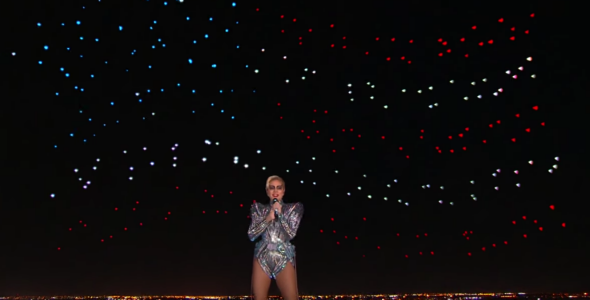
\includegraphics[width=12cm]{figures/super_bowl.png}
	\caption{Lady Gaga 300 drónnal a háttérben a 2017-es Super Bowl döntőjének félideje alatti koncerten \cite{super-bowl-pic}}
	\label{fig:super-bowl}
\end{figure}
Persze ebben a példában egy pár perces feladatról beszélünk az irányított robotok számára, a felhős megoldással pedig egy hosszútávú optimalizációt szeretnénk megadni.

\section{Használt kifejezések}
A hálózati-, virtualizációs- és robotiparban rengeteg rövidítés, mozaikszó és kifejezés létezik, amit főként csak azok ismernek, akik
jelentősebben mélyültek el ezen iparág területén. Két csoportra bontom a diplomatervemhez használt kifejezéseket:
\begin{enumerate}
	\item Azon szakmai kifejezések, amik elterjedtek a mérnöki szakmákban és mondjuk a BME VIK tetszőleges hallgatója, bármely, nem infokommunikációs szakosodás mellett is nagy valószínűséggel ismer és nem kell ismertetnem a tanulmányban. Pár példa a kategóriában, amikre külön nem térek ki, nem oldom fel a szövegben, ilyenek az IPv4, NAT, hálózati réteg, HTTP, CPU, for ciklus.
	\item Azokat a kifejezéseket amik pedig a témához, szakterülethez kapcsolódnak, például a kifejezetten hálózati kommunikáció, virtualizáció, robot, irányítás iparágakba tartozó kifejezések, amiket nem általános mérnöki ismeretek, azokat a szövegben az első használatnál kifejtem, továbbá itt összegyűjtöm.
\end{enumerate}
A tanulmányban használt speciális kifejezések:
\begin{itemize}
	\item QoS (Quality of Service) - A szolgáltatás minőségének a biztosítása
	\item Virtuális gép (Virtual Machine, VM) - Virtualizált önálló teljes értékű operációs rendszer gazdagépen (host-on)
	\item KVM (Kernel-based Virtual Machine) - Kernelhez elosztott időben hozzáférő virtuális gép
	\item Host OS - Hosted virtualizáció esetén a gazdaoperációs rendszer
	\item Guest OS - Hosted virtualizált operációs rendszer a host OS fölött
	\item Hypervisor - A hardveren való virtualizációt megvalósító szoftver
	\item Node - A felhőrendszer egy fizikai eszköze
	\item Cluster - A felhőrendszerbe csatolt fizikai eszközök kapcsolata
	\item Volume - Szolgáltatás/VM háttértára
	\item Vertikális skálázás - Node hozzáadása a cluster-hez
	\item Horizontális skálzás - Node fejlesztés
	\item GCS (Ground Control Station) - Földi irányítóállomás
\end{itemize}